\documentclass[12pt]{article}
\usepackage[margin=1in]{geometry}
\usepackage{amsmath}
\usepackage{graphicx}
\usepackage{float}
\usepackage{enumitem}
\usepackage{booktabs}
\usepackage{tikz}
\usepackage{fancyhdr}
\usepackage[rgb]{xcolor}
\usepackage{tcolorbox}
\usepackage{wrapfig}

% Define colors
\definecolor{labblue}{RGB}{51,101,138}
\definecolor{safetyyellow}{RGB}{255,240,150}
\definecolor{conceptgreen}{RGB}{200,230,201}

% Logo configuration
\newcommand{\headerlogo}[1]{%
    \includegraphics[height=20pt]{#1}%
}

% Configure page style
\pagestyle{fancy}
\fancyhead{}
\fancyhead[L]{\headerlogo{cinec_logo.png} \hspace{1em} Physics Laboratory}
\fancyhead[R]{Newton's Second Law}
\fancyfoot{}
\fancyfoot[C]{\thepage}

\begin{document}

\begin{center}
{\Large \textbf{Laboratory Investigation E1:}}\\[0.5cm]
{\LARGE \textbf{Newton's Second Law}}\\[1cm]
\rule{\textwidth}{0.4pt}
\end{center}



\section*{Experimental Overview}

 \textbf{Key Concept}:\\
 Newton's Second Law reveals a profound relationship between force, mass, and motion: The acceleration of an object is directly proportional to the net force acting on it and inversely proportional to its mass. Mathematically, we express this as: $$\vec{F} = m\vec{a}$$

This investigation explores three fundamental relationships that together illuminate the elegant mathematical structure of motion:

\begin{enumerate}[label=\arabic*.]
\item The linear relationship between force and acceleration (constant mass)
\item The inverse relationship between mass and acceleration (constant force)
\item The linear relationship between acceleration and reciprocal mass (constant force)
\end{enumerate}

Using specialized physics software, we'll measure accelerations directly as we systematically vary forces and masses, revealing the mathematical patterns that govern motion at the most fundamental level.

\begin{tcolorbox}[colback=conceptgreen!10,colframe=conceptgreen,title=\textbf{Investigation Strategy}]
Our approach mirrors the scientific method at its best: we'll isolate and study each variable's influence by holding others constant. This method of controlled variation lets us discover how each factor contributes to the overall behavior of the system.
\end{tcolorbox}

\section*{Materials and Equipment}
\begin{itemize}
\item Dynamics track with motion sensor
\item Dynamics cart (mass ≈ 0.180 kg)
\item Set of 5g masses for hanging
\item Pulley system
\item Computer with experiment software and Excel
\item String (approximately 1m)
\end{itemize}

\section*{Safety Considerations}
\begin{tcolorbox}[colback=safetyyellow!30,colframe=safetyyellow!80,title=\textbf{Safety Protocol}]
\begin{itemize}
\item Secure the track firmly to prevent tipping
\item Verify pulley alignment before starting
\item Handle masses carefully to prevent dropping
\item Keep fingers clear of moving parts
\item Ensure string is properly tied to prevent masses from falling
\end{itemize}
\end{tcolorbox}

\section*{Part 1: Force and Acceleration}

 \textbf{Investigation Focus}:\\
 We examine how acceleration changes when we vary the applied force while keeping mass constant. The software directly measures the cart's acceleration for each applied force.

\section*{Experimental Setup}
\begin{center}
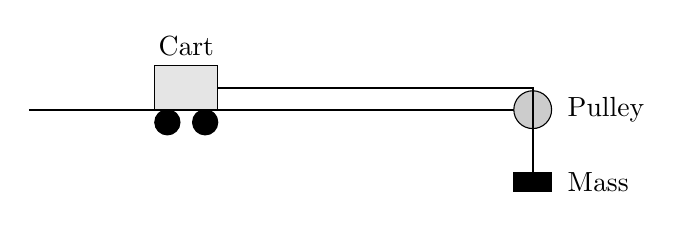
\begin{tikzpicture}[scale=0.8]
% Draw track
\draw[thick] (0,2) -- (8,2);
% Draw cart
\draw[fill=gray!20] (2,2) rectangle (3,2.7);
\draw[fill=black] (2.2,1.8) circle (0.2);
\draw[fill=black] (2.8,1.8) circle (0.2);
% Draw pulley
\draw[fill=gray!40] (8,2) circle (0.3);
% Draw string and mass
\draw[thick] (3,2.35) -- (8,2.35) -- (8,1);
\draw[fill=black] (7.7,0.7) rectangle (8.3,1);
% Labels
\node[above] at (2.5,2.7) {Cart};
\node[right] at (8.4,2) {Pulley};
\node[right] at (8.4,0.85) {Mass};
\end{tikzpicture}
\end{center}

\section*{Procedure}
\begin{enumerate}[label=\arabic*.]
\item Level the track using the adjustable feet
\item Measure and record the cart's mass ($M_c$)
\item Attach the string to the cart and over the pulley
\item Add a 5g mass (0.005 kg) to the hanging end
\item Calculate the applied force: $F = mg = 0.005\text{ kg} \times 9.81\text{ m/s}^2 = 0.049\text{ N}$
\item Start the data collection in the software
\item Record the measured acceleration
\item Add another 5g mass
\item Repeat steps 5-7 until you have data for all five masses (3-5 measurements each mass)
\end{enumerate}

\section*{Data Collection}
Record your measurements in this format:

\begin{table}[H]
\centering
\begin{tabular}{ccc}
\toprule
Hanging Mass & Applied Force & Measured Acceleration \\
(kg) & (N) & (m/s²) \\
\midrule
0.005 & 0.049 & \\
0.010 & 0.098 & \\
0.015 & 0.147 & \\
0.020 & 0.196 & \\
0.025 & 0.245 & \\
\bottomrule
\end{tabular}
\end{table}

> \textbf{Data Pattern Note}:\\
> Each 5g increase in hanging mass adds exactly 0.049 N of force, creating a systematic progression ideal for discovering mathematical relationships.

\section*{Part 2: Mass and Acceleration}

> \textbf{Investigation Focus}:\\
> We now explore how acceleration changes with mass while keeping force constant. This reveals the inverse relationship at the heart of Newton's Second Law.

\section*{Procedure}
\begin{enumerate}[label=\arabic*.]
\item Keep the hanging mass constant at 10g (0.098 N)
\item Start with the original cart mass
\item Record the acceleration
\item Add a 50g mass to the cart
\item Record the new acceleration
\item Repeat steps 4-5 for four more measurements
\end{enumerate}

\section*{Data Collection}
Record your results in this format:

\begin{table}[H]
\centering
\begin{tabular}{ccc}
\toprule
Cart + Added Mass & Force & Acceleration \\
(kg) & (N) & (m/s²) \\
\midrule
0.1826 & 0.098 & \\
0.2326 & 0.098 & \\
0.2826 & 0.098 & \\
0.3326 & 0.098 & \\
0.3826 & 0.098 & \\
\bottomrule
\end{tabular}
\end{table}

\section*{Part 3: Advanced Analysis}

> \textbf{Mathematical Insight}:\\
> By plotting acceleration versus 1/m, we transform the inverse relationship into a linear one, revealing another face of Newton's Second Law.

Create a new column in your spreadsheet for 1/m and plot a vs. 1/m. The slope of this line should equal your applied force.

\section*{Data Analysis in Excel}

\begin{tcolorbox}[colback=labblue!5,colframe=labblue,title=\textbf{Creating Effective Scientific Graphs}]
For each relationship, create a scatter plot:
\begin{enumerate}[label=\arabic*.]
\item Select appropriate columns for x and y axes
\item Insert → Scatter Plot
\item Add clear axis labels with units
\item Include a descriptive title
\item Add a trendline and display its equation
\end{enumerate}

\textbf{Expected Relationships:}
\begin{itemize}
\item F vs. a: Linear with slope = 1/m
\item m vs. a: Inverse (hyperbolic)
\item 1/m vs. a: Linear with slope = F
\end{itemize}
\end{tcolorbox}


\section*{Discussion Questions}
\begin{enumerate}[label=\arabic*.]
\item How does doubling the force affect acceleration? Is this what you'd expect from $F = ma$?
\item Why does acceleration decrease as we add mass to the cart?
\item What physical meaning does the slope have in each graph?
\item How do your results support or challenge Newton's Second Law?
\item What sources of systematic error might affect your results?
\item How could this experiment be improved?
\end{enumerate}

\section*{Conclusion Guidance}
Your lab report conclusion should synthesize:

\begin{itemize}
\item The three mathematical relationships discovered
\item How well your data supports Newton's Second Law
\item Major sources of experimental uncertainty
\item Connections between theory and experiment
\item Suggestions for experimental improvements
\end{itemize}

> \textbf{Final Reflection}:\\
> Consider how Newton's insight about force, mass, and acceleration reveals fundamental patterns in nature. These relationships govern everything from the motion of atoms to the orbits of planets.

\end{document}